% \input{Functional}

\subsection{Functional Viewpoint}

\begin{itemize}
\item Related stakeholders: KLM, Initiator, EU-Claim
\item Related Concerns: Users of the system, Available functionality to each user group, Grouping functionalities
\item Related design decisions: Flight-Information (p. \pageref{dd:flight-inf}); Billing module (p.~\pageref{sec:minor-dd}), Update or edit reviews (p.~\pageref{sec:minor-dd})
\end{itemize}

\newpage
\begin{landscape}
\begin{figure}
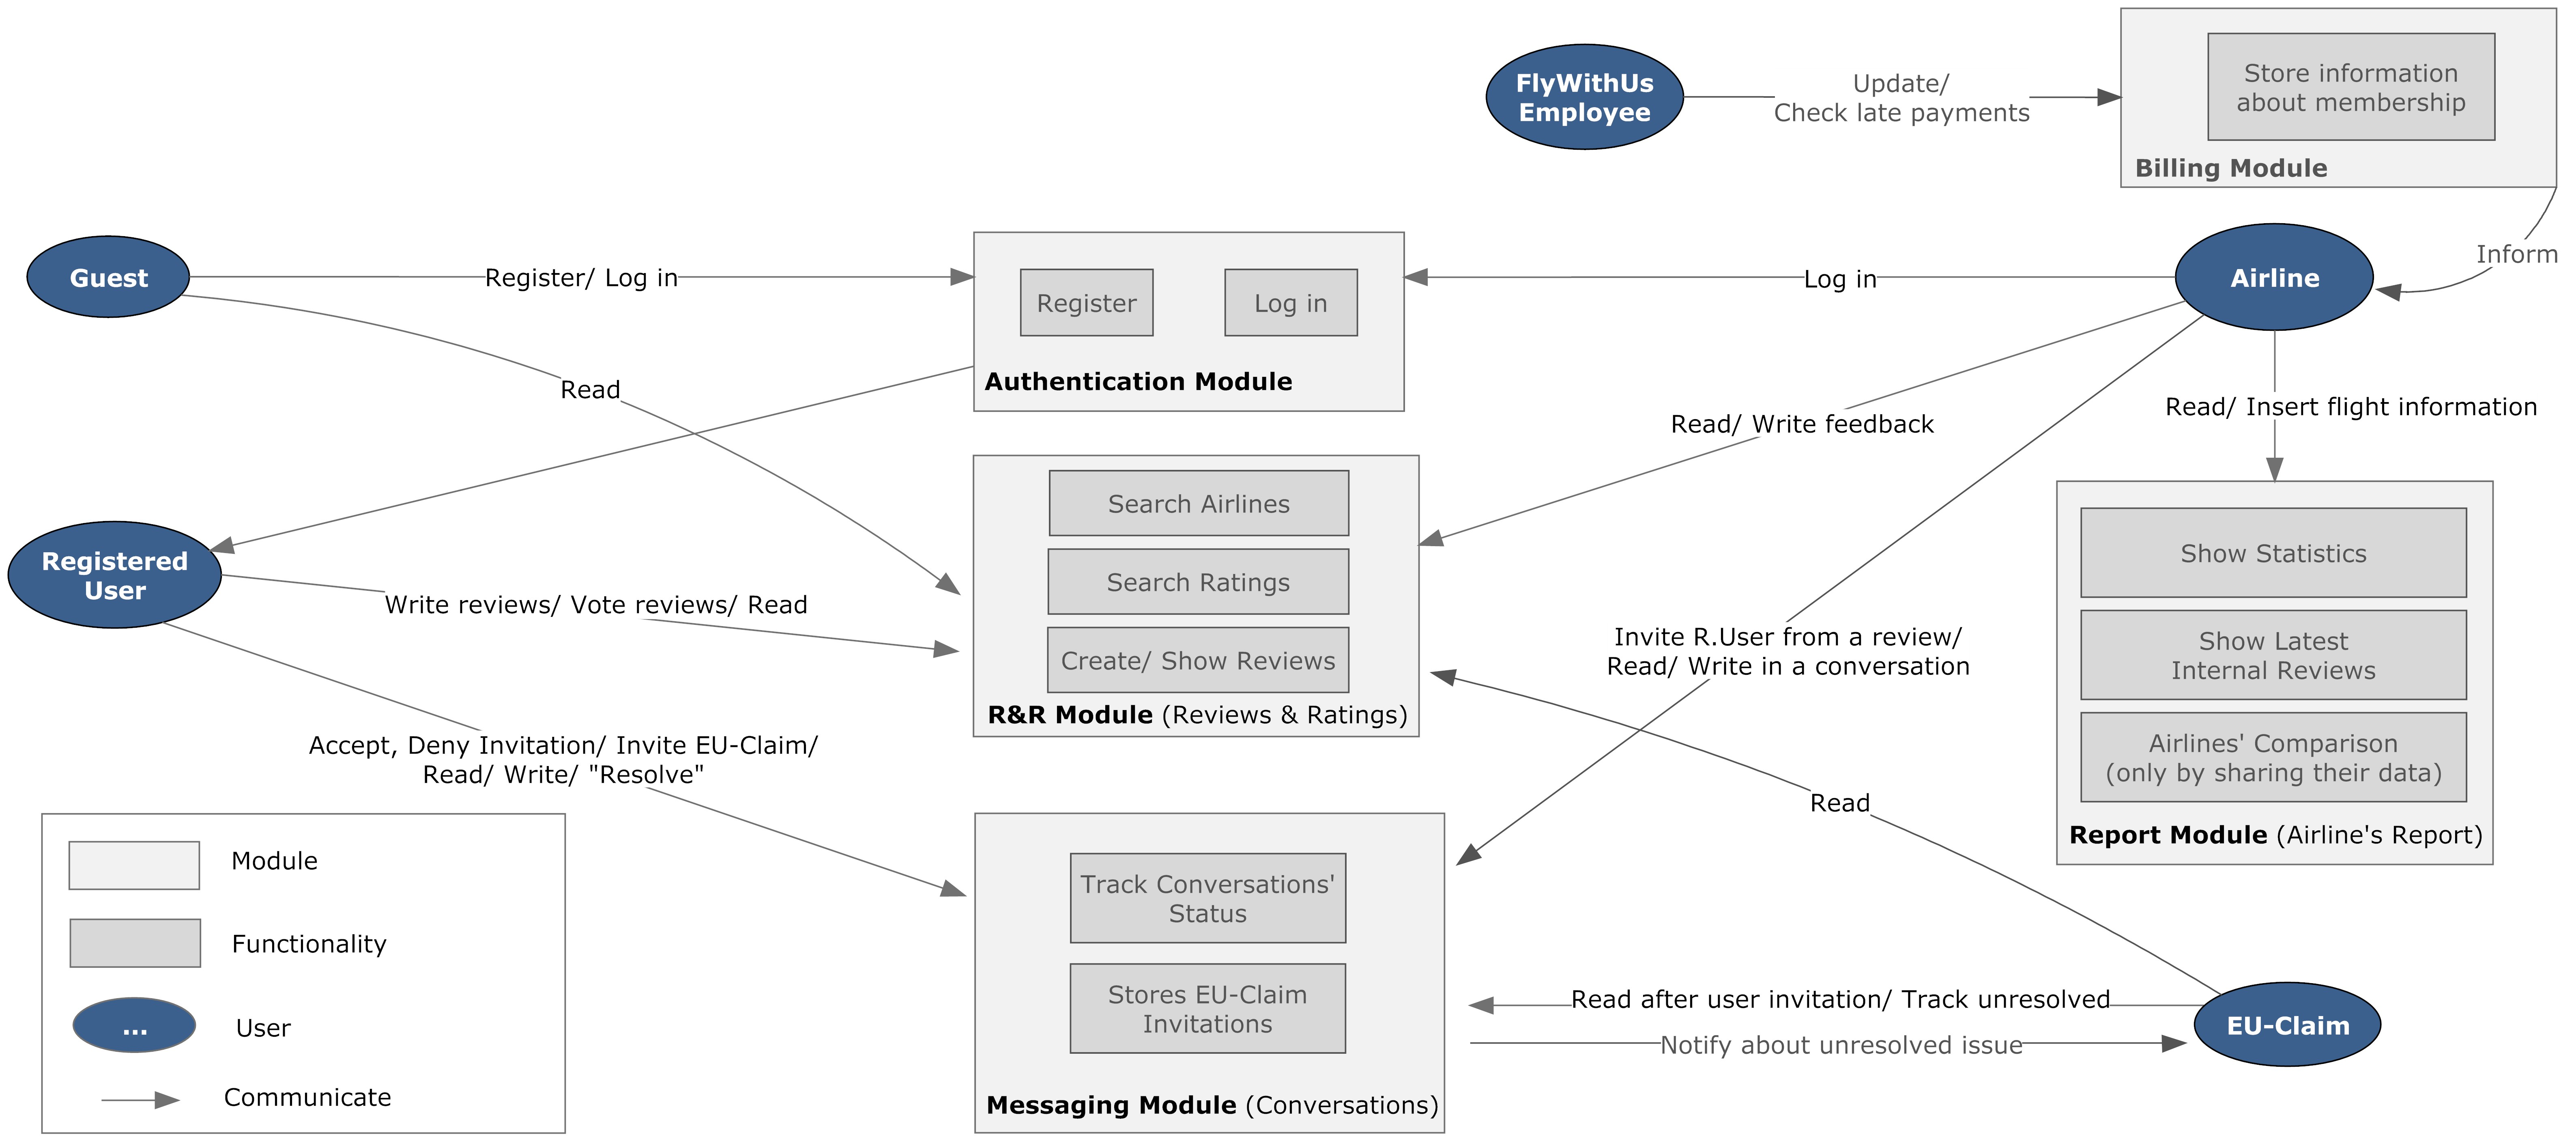
\includegraphics[width=600px]{Functional_Viewpoint.jpg}
\caption{Functional Viewpoint}
\label{fig:functional}
\end{figure}
\end{landscape}

The functional viewpoint (Figure~\ref{fig:functional}) illustrates the functionality supported by the system and its connections to the users. The direction of the arrows shows who or what initiates this connection, for example EU-Claim can monitor a conversation (initiated by EU-Claim) but  the system notifies EU-Claim about an issue that has been unresolved for a configurable period of time (initiated by Messaging module). The functionalities that are based in the same entities of the system are grouped together to help the reader understand their connections. For example, all the functionalities  provided only to airlines are included in a {\em report} as a result these functionalities are grouped in the Report module. The association between the modules presented in the viewpoint and the functional requirements listed in appendix~\ref{sec:requirements} are presented in following table.
%TODO: Fix reference

\begin{longtable}{| l | l | l |}
\hline
\label{tab:associateSysReq} 
\textbf{Requirement} & \textbf{System} & \textbf{Users} \\ \hline
Show ratings & Review System & Guests, Registered Users \\ \hline
Post/Read/Search & Review System & Registered Users \\ \hline
Messaging & Messaging System & Registered Users, Airlines, EUC \\ \hline
Reporting  & Reporting System & Airlines \\ \hline
Statistics & Reporting System & Airlines \\ \hline 

\end{longtable}

Furthermore, the viewpoint presents the availability of the functionalities to each user group and the communication between these groups through the system. For instance, a guest can register or log in the system and  become a registered user, or an airline can invite a user to a private conversation in order to resolve a potential complaint; then the user can accept the invitation and he can  also invite EU-Claim to monitor their conversation to ensure the integrity of this process. Each entity presented in the viewpoint is discussed in the following subsections.

\subsubsection{Users}
\paragraph{Guests.} A guest is a user of the system with no account. He can read reviews and search for ratings using the R\&R module. Furthermore, a guest can  register or log in using the Authentication module.

\paragraph{Registered User.} A registered user can read, write and vote reviews and can search for rating using the R\&R module. Additionally, he can communicate with an airline through the Messaging module in private, meaning that other parties  (except for EU-Claim and only if it is invited) cannot read this conversation.

\paragraph{Airlines.} An airline represents the airlines that have payed membership in FlyWithUs. The progress of an airline can be monitored through the Report module. Also an airline can see statistics, ratings and can advance search through the database by providing flight information and correlating the search results. Additionally, airlines can see their progress in comparison with other airlines if they agree to share their information.

Moreover, as far as customer satisfaction is concerned, an airline can write feedback to a review posted on the R\&R module or invite a user to a private conversation through the Messaging module. Finally, an airline can be informed about the status of the membership through the Billing module.

\paragraph{EU-Claim.} In order to ensure the integrity of the system, separate accounts will be provided to EU-Claim in order to be able to  monitor conversations when invited and also to be notified about a conversation if it is unresolved for a configurable period of time. Finally, EU-Claim will be able to search for ratings through the R\&R module.

\paragraph{FlyWithUs Employee.} FlyWithUs employee is an employee of FlyWithUs whose responsibility is to update or check the membership status of the airlines' according to their payments.

\subsubsection{Modules}
\paragraph{Review \& Rating Module.} This module is responsible for inserting new internal reviews on the system, handling the votes on reviews and provides the search interface to the registered users and the guests. This module allows searching according to specific categories of ratings, for example which airline has the best food or the best client support, or according to general ratings. 

The R\&R module does not allow the users to  edit or delete their reviews in order to preserve the system's consistency and fairness.

\paragraph{Report Module.} This module provides the tools to the airlines to monitor their progress. It shows statistics about an airline's progress, the latest reviews on FlyWithUs and also allows the airline to use advance search, which can provide better parametrization, for example search according to flight information. Finally, if airlines can declare that they want to share their information from gathered from the system with other airlines. In that case, the airlines can also see a comparison between their progress and the progress of other airlines.

\paragraph{Messaging Module.} This module is responsible for the private conversations between the registered users and the airlines. At first, an airline wishes to contact the author of a review, then the author is invited to a private conversation by the Messaging module. If the author accepts it can invite EU-Claim to monitor this conversation through this module. Additionally, this module keeps track of all the resolved and unresolved issues, it can provide statistics and it can also notify EU-Claim if a conversation has been unresolved for a configurable (by EU-Claim) period of time. Only the affiliated parties of a conversation can read this conversation as a result the Messaging module checks the identity of the user before it grants him access.

\paragraph{Billing Module.} This module is responsible for keeping track of the membership status of the airlines. It will notify both the FlyWithUs employee and the associated airline if there is a late payment and in case that the airline's membership is not renewed it will revoke the airline's access to the Reporting module. (Minor design decisions~\ref{sec:minor-dd})

\paragraph{Authentication Module.} This module is responsible for the registration of new users and for signing in existing users and identifying their type.
